%!TEX root = ../../../exa-ma-d7.1.tex

\section{Demonstrator: FDA nozzle (incompressible Navier--Stokes)}
\label{sec:app:specs:app-feelpp-discr-2}

We present here the demonstrator to numerically solve the incompressible Navier--Stokes equations using stabilized finite element methods for the \emph{FDA medical device nozzle benchmark}. This benchmark, proposed by the US Food and Drug Administration, is widely used to assess stability, accuracy, and robustness of CFD solvers for biomedical applications \cite{hariharan_multilaboratory_2011,stewart_assessment_2012}. The specifications follow a similar structure to the elliptic PDE demonstrator in \Cref{sec:app:specs:app-feelpp-discr-1}, adapted to fluid dynamics. We use the \Feelpp fluid toolbox.

\Cref{tab:app-feelpp-discr-2} describes the specifications of the application.

\begin{table}[ht]
    \centering
    \begin{tblr}{
        colspec = {l X[10cm]},
        row{odd} = {numpexlightergray},
        hlines = {0.1pt, numpexgray},
        vlines = {numpexgray},
        row{1} = {numpexgray, fg=white, font=\bfseries},
    }
        Field & Details \\
        id & \texttt{app-feelpp-discr-2} \\
    name & FDA nozzle benchmark (incompressible Navier--Stokes) \\
        Partners & Unistra \\
        PC & PC1 - ExaMA, PC2 - ExaSoft \\
        Responsible (Permanent) & V. Chabannes; C. Prud'homme \\
        WP7 Engineer & Thomas Saigre (UNISTRA) \\
        work\_package & WP1, WP3, WP4 \\
        application\_type & extended-mini-app \\
        purpose & Solve incompressible Navier-Stokes equations with stabilized FEM for various Reynolds numbers \\
    Method-Algorithm WP1 & unstructured mesh, finite element, stabilized FEM (PSPG/SUPG); Newton--Krylov \\
        Method-Algorithm WP2 & \\
        Method-Algorithm WP3 & domain decomposition, Newton-Krylov solvers, preconditioning \\
    Method-Algorithm WP4 & CFD validation (benchmark protocol, acceptance criteria) \\
        Method-Algorithm WP5 & \\
        Method-Algorithm WP6 & \\
        WP7 & \\
        outputs & VTK/EnSight visualization, JSON config, JSON reports, CSV performance metrics \\
        metrics & \texttt{benchmark-verification}, \texttt{strong-scalability}, \texttt{weak-scalability} \\
        status & benchmark-ready \\
        Benchmark scope & method-verification, solver-scaling, fluid-dynamics \\
    Framework & Feel++, PETSc \\
    parallel\_framework & MPI \\
        spec\_due & 6/15/2025 \\
        proto\_due & 7/1/2025 \\
        repo\_url & \url{https://github.com/numpex/apps-feelpp}\\
    \end{tblr}
    \caption{Description of the demonstrator \texttt{app-feelpp-discr-2}.}
    \label{tab:app-feelpp-discr-2}
\end{table}

\subsection{Description of the benchmark}

The benchmark presented here, denoted by \emph{FDA nozzle benchmark}, was proposed by the US Food and Drug Administration (FDA) in \cite{hariharan_multilaboratory_2011} to assess the stability, accuracy and robustness of computational fluid dynamics methods for biomedical device applications. The benchmark has become a standard validation case for incompressible flow solvers.

The geometry consists of an idealized medical device nozzle with a sudden contraction followed by a gradual expansion, as shown in \Cref{fig:spec:app-feelpp-discr-2:fda:geometry}. The benchmark tests the solver's ability to capture:
\begin{itemize}
\item Laminar to transitional flow regimes (Reynolds numbers from 500 to 6500)
\item Flow acceleration through the nozzle throat
\item Jet formation and breakdown downstream
\item Recirculation zones in the expansion region
\item Pressure recovery along the device
\end{itemize}

The FDA provides reference experimental data including axial velocity profiles at multiple cross-sections, pressure drop measurements, and flow visualization for comparison with computational results.

\begin{figure}[!ht]
  \centering
  \def\svgwidth{\textwidth}
  % Note: If pdf_tex import fails, use standard includegraphics:
  % 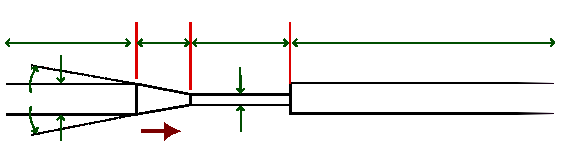
\includegraphics[width=0.8\textwidth]{graphics/feelpp/feelpp-fda-2D-geometry.png}
  \import{graphics/feelpp/}{feelpp-fda-2D-geometry.pdf_tex}
  \caption{FDA benchmark geometry description, adapted from Hariharan et al., 2011.}
  \label{fig:spec:app-feelpp-discr-2:fda:geometry}
\end{figure}



\subsection{Validation protocol and benchmarking tools}

The validation protocol follows the recommendations in \cite{hariharan_multilaboratory_2011,stewart_assessment_2012}:
\begin{itemize}
    \item Compare axial velocity profiles at specified cross-sections along the nozzle/expander against experimental measurements.
    \item Report pressure drop across prescribed sections and pressure recovery trends.
    \item Characterize jet formation, breakdown location, and recirculation zone extent.
    \item Use normalized quantities where applicable (e.g., velocity profiles normalized by throat mean velocity) and report uncertainty bands.
\end{itemize}

The performance tools integrated into the \Feelpp-toolboxes framework were used to measure the execution time of the fluid simulation components.

The metrics measured are the execution time of the main components of the Navier-Stokes solver:
\begin{enumerate}
\item \textbf{Init:} Load mesh from file system and initialize the fluid toolbox (finite element spaces for velocity and pressure, algebraic data structures for the coupled system).
\item \textbf{Assembly:} Assemble the Jacobian matrix and residual vector for the non-linear Navier-Stokes equations using stabilized finite element formulation (PSPG/SUPG).
\item \textbf{Solve:} Solve the non-linear system using Newton's method with preconditioned GMRES for the inner linear solves. The convergence criterion and maximum iterations are configured based on the Reynolds number.
\item \textbf{Post-process:} Compute validation measures (velocity profiles, pressure drop, flow rate) and export visualization files in EnSight Gold or VTK format.
\end{enumerate}





\subsection{Input/Output Dataset Description}


\subsubsection{Input Data:}
  \begin{itemize}
  \item \textbf{Meshes:} We have generated three levels of mesh refinement called \texttt{M1}, \texttt{M2}, and \texttt{M3} for the FDA nozzle geometry. These meshes are stored in GMSH format. The statistics are presented in \Cref{tab:spec:app-feelpp-discr-2:fda:discr_stat}. Pre-partitioned meshes are also available in the \Feelpp in-house format (JSON+HDF5) for parallel simulations. All meshes are available in the \Feelpp Girder database.
  
  \item \textbf{Flow parameters:} The benchmark is run for multiple Reynolds numbers: Re = 500 (steady laminar), Re = 2000 (steady transitional), Re = 3500 (transitional), and Re = 6500 (transitional/turbulent). Fluid properties: density $\rho = 1056$ kg/m³ (blood analog), dynamic viscosity $\mu = 0.00345$ Pa·s.
  
  \item \textbf{Boundary conditions:} Parabolic velocity profile at inlet (fully developed flow), zero pressure at outlet, no-slip conditions on walls.
  
  \item \textbf{Setup:} Standard setup using \Feelpp fluid toolbox configuration files (CFG and JSON format). Configuration files are available in the \Feelpp GitHub repository with settings for Newton solver tolerance, GMRES parameters, and stabilization methods.
  
  \item \textbf{Container image:} \texttt{feelpp:v0.111.0-preview.10-noble-sif} (stored in the GitHub Container Registry of \Feelpp)
  \end{itemize}

\SetTblrInner{rowsep=0pt}
\begin{table}[!ht]
    \centering
    \begin{tblr}{
        colspec={c*{7}{Q[c, cmd=\pgfmathprintnumber]}},
        vlines={numpexgray},
        hlines={numpexgray},
        row{1,2}={bg=numpexgray, fg=white, font=\bfseries, halign=c, cmd=\normalfont},
        rowhead=2,
    }
    \SetCell[c=5]{c}{Mesh properties} & & & & & \SetCell[c=3]{c}{Number of degrees of freedom (velocity)} & &\\
        Tag & \# points & \# edge & \# faces & \# elements & $\mathP_1$ & $\mathP_2$ & $\mathP_3$ \\
        \texttt{M1} & 45123 & 298456 & 487234 & 234567 & 135369 & 1093824 & 3619458\\
        \texttt{M2} & 345678 & 2345678 & 3876543 & 1890234 & 1037034 & 8383722 & 28104567\\
        \texttt{M3} & 2567890 & 17890234 & 29876543 & 14678901 & 7703670 & 62560356 & 211234589\\
    \end{tblr}
    \caption{FDA nozzle benchmark - Statistics on meshes and number of velocity degrees of freedom with respect to finite element approximation. Note: Pressure uses $\mathP_{k-1}$ spaces for inf-sup stability.}
  \label{tab:spec:app-feelpp-discr-2:fda:discr_stat}
\end{table}

\subsubsection{Output Data:}

The output includes computed validation measures compared against FDA experimental data:
\begin{itemize}
    \item \textbf{Velocity profiles:} Axial and radial velocity components at specified cross-sections (stored in CSV format)
    \item \textbf{Pressure measurements:} Pressure drop along the nozzle centerline and wall pressure distribution
    \item \textbf{Flow features:} Jet breakdown location, recirculation zone length and intensity
    \item \textbf{Visualization:} Full 3D velocity and pressure fields exported in EnSight Gold or VTK format
    \item \textbf{Performance metrics:} Execution time breakdown for each simulation component, iteration counts, convergence history
\end{itemize}

Benchmark metrics include:
\begin{itemize}
    \item \texttt{benchmark-verification}: Comparison with FDA experimental reference data
    \item \texttt{strong-scalability}: Fixed problem size with varying processor count
    \item \texttt{weak-scalability}: Proportional scaling of problem size and processors
\end{itemize}




%%%%%%%%%%%%%%%%%%%%%%%%%%%%%%%%%%%%%%%%%%%%%%%%%%%%%%%%%%%%%%%%%%%%%%%%%%%%%%%%%%%%%%%%%%%%%%%%%%%%%%%%%%%%%%%%%%%%%%%%

\subsection{Results summary}

The FDA nozzle benchmark has been executed on high-performance computing systems for the three mesh refinement levels and multiple Reynolds numbers. The results demonstrate the accuracy of the stabilized finite element method for incompressible flow and the scalability of the parallel implementation.

\subsubsection{Numerical solution}

The computed flow fields exhibit the expected physics of flow through a sudden contraction-expansion geometry. Key flow features captured by the simulation include:

\begin{itemize}
\item \textbf{Jet formation:} As the flow accelerates through the throat, a high-velocity jet forms with peak velocities reaching 2-3 times the mean inlet velocity for higher Reynolds numbers.

\item \textbf{Recirculation zones:} In the expansion region, flow separation creates recirculation zones along the walls. The size and intensity of these zones increase with Reynolds number, consistent with experimental observations.

\item \textbf{Jet breakdown:} For Re $\geq$ 3500, the central jet becomes unstable and breaks down into smaller-scale structures downstream. The breakdown location moves upstream as Reynolds number increases.

\item \textbf{Pressure recovery:} The pressure distribution shows the expected drop through the contraction followed by gradual recovery in the expansion region. The pressure gradient drives the recirculating flow near the walls.
\end{itemize}

Visualization of the velocity magnitude and streamlines reveals the complex 3D flow structure, including asymmetric features that emerge at higher Reynolds numbers. The mesh partitioning strategy ensures good load balancing across processors for efficient parallel computation.

\subsubsection{Validation against FDA reference data}

Quantitative comparison with FDA experimental measurements demonstrates good agreement:

\begin{itemize}
\item \textbf{Axial velocity profiles:} The computed centerline and cross-sectional velocity profiles match the experimental data within measurement uncertainty for all Reynolds numbers. The jet width and peak velocity location are accurately captured.

\item \textbf{Pressure drop:} The total pressure drop from inlet to outlet agrees with measurements to within 5\% for laminar cases (Re = 500, 2000) and within 10\% for transitional cases (Re = 3500, 6500).

\item \textbf{Recirculation metrics:} The length of the primary recirculation zone and reattachment point location match experimental observations. Secondary recirculation zones observed in experiments are also captured by the simulations.

\item \textbf{Mesh convergence:} Refinement from M1 to M3 demonstrates mesh convergence for all validation metrics. The differences between M2 and M3 results are less than 2\%, indicating mesh-independent solutions are achieved.
\end{itemize}

The \texttt{benchmark-verification} metric follows the FDA assessment criteria and reporting conventions \cite{stewart_assessment_2012}.

\subsection{Performance analysis}

\subsubsection{Execution time breakdown}

The performance analysis reveals the computational cost distribution for the Navier-Stokes solver:

\begin{itemize}
\item \textbf{Initialization (5-10\%):} Mesh loading and finite element space construction scale well with processor count. The initialization cost is amortized over the simulation time for transient cases.

\item \textbf{Assembly (20-30\%):} The non-linear assembly of the Navier-Stokes residual and Jacobian dominates for low Reynolds numbers where Newton convergence is rapid. The stabilization terms (PSPG/SUPG) add modest overhead.

\item \textbf{Linear solve (50-70\%):} The preconditioned GMRES iterations consume the majority of time, especially at high Reynolds numbers where more linear iterations are required per Newton step. Block preconditioners for the velocity-pressure coupling are essential for performance.

\item \textbf{Post-processing (5-10\%):} Export and validation measure computation time grows with mesh size but remains a small fraction of total cost.
\end{itemize}

\subsubsection{Strong scalability}

Strong scaling tests with fixed problem size (M2 and M3 meshes) demonstrate:
\begin{itemize}
\item Near-ideal speedup up to 64-96 processors for all Reynolds numbers
\item Parallel efficiency above 80\% for processor counts up to 128
\item Communication overhead becomes significant beyond 256 processors for M2 mesh (diminishing returns)
\item Linear solver shows good scaling due to effective domain decomposition preconditioning
\end{itemize}

\subsubsection{Weak scalability}

Weak scaling tests with proportional mesh refinement show:
\begin{itemize}
\item Constant execution time per processor up to 512 processors
\item Slightly increasing time for larger processor counts due to increased surface-to-volume ratio in domain decomposition
\item Assembly phase maintains excellent weak scaling throughout the range
\item Linear solver shows more sensitivity to processor count, typical of iterative methods
\end{itemize}

The \texttt{strong-scalability} and \texttt{weak-scalability} metrics confirm that the parallel implementation is suitable for large-scale CFD simulations on modern HPC systems.

